% Use a one-sided article template
\documentclass[oneside]{article}
% Decrease the margins a little
\usepackage{fullpage}

% Set up for including graphics
% We'll use png or pdf graphics
\usepackage[pdftex]{graphicx}
\DeclareGraphicsExtensions{.png,.pdf}

% Hyperref adds hyperlinks to the document automatically
% It's not much use yet, but it will be
\usepackage{hyperref}

% For including code into the document
\usepackage{verbatim}

% Tweak the default fonts a little
\renewcommand\rmdefault{bch}
\usepackage[small]{caption}
\usepackage[small]{titlesec}
\linespread{1.07} 

\raggedbottom
\pagestyle {empty}

\begin{document}

\begin{center}
\textbf{Stat640 - Progress Report 2 - Charlemagne and the Carolingian Empire (Delhey/Portman)}
\end{center}

\begin{center}
  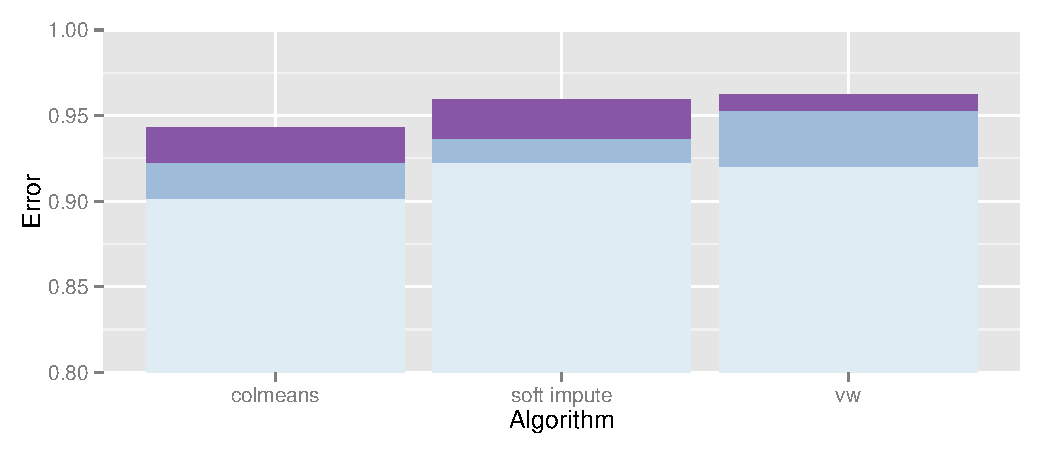
\includegraphics[width = 0.75\linewidth]{vis}
\end{center}

\begin{description}
\item[What learning algorithms have you tried?] 
Since the last progress report we've focused on implementing two general types of learning algorithms: matrix factorization and k-nearest neighbors. Our original goal for this project report was to have a successful (i.e. reasonable error) submission for both of these learning algorithms as well as a simple ensemble of these two methods.

We had some success with matrix factorization. We were able to implement a matrix completion model using the nuclear-norm regularization on the SVD as we discussed in class, using cross-validation to select the best regularization parameter.

We found less success with k-nearest neighbors. Our first attempt was to calculate the Pearson correlation between the normalized rows and columns. This approach was both an unwieldy computation and an over-estimator of similarity between users/movies that had very few ratings. We're currently exploring other alternatives for approximating similarity both item-wise and user-wise, but computation remains a problem. As such, we've yet to meet our goal of a successful k-nearest neighbors submission.

\item[Performance. Which algorithms worked well? Which performed poorly? Why?]
Our matrix factorization approach has performed the best for us so far. This isn't too surprising given the renowned success of the SVD to collaborative filtering problems similar to ours. 

We suspect that our k-nearest neighbors approach with appropriate prepossessing and  value of \verb|k| would score comparably to our matrix completion. 

We also suspect that our blend or ensemble of these two methods would score reasonably better than just matrix factorization alone. Indeed, literature on the topic notices how these two methods complement each other on similar sparse datasets. At the same time, we suspect that even such an ensemble would most likely not place us at the front of the leader-board and so cannot be our only move forward. 

\item[Project organization and innovation.] 
Our project organization has remained more or less the same since the last project report. Our level of innovation, however, is a bit more vague. On the one hand, we are still working on implementing many of the methods in the literature. On the other hand, we are operating a higher level of sophistication on our problem than we were one month ago. As we approach the end of the competition and begin to push the limits of our methods as discussed specifically in the literature we hope to make some novel improvements to our methods. 

\item[What are the future direction in which you would like to go?]
One future direction that we would like to move towards is utilizing the additional data outside of the ratings matrix. The literature on the Netflix prize seems to indicate that proper utilization of this additional user and movie data (although our additional data is in many important ways different) is key to getting a great score.


\end{description}

\end{document}